\documentclass[utf8x]{beamer}

\mode<presentation> {

% The Beamer class comes with a number of default slide themes
% which change the colors and layouts of slides. Below this is a list
% of all the themes, uncomment each in turn to see what they look like.

%\usetheme{default}
%\usetheme{AnnArbor}
%\usetheme{Antibes}
%\usetheme{Bergen}
%\usetheme{Berkeley}
%\usetheme{Berlin}
%\usetheme{Boadilla}
%\usetheme{CambridgeUS}
%\usetheme{Copenhagen}
%\usetheme{Darmstadt}
%\usetheme{Dresden}
%\usetheme{Frankfurt}
%\usetheme{Goettingen}
%\usetheme{Hannover}
%\usetheme{Ilmenau}
%\usetheme{JuanLesPins}
%\usetheme{Luebeck}
%\usetheme{Madrid}
%\usetheme{Malmoe}
%\usetheme{Marburg}
%\usetheme{Montpellier}
%\usetheme{PaloAlto}
%\usetheme{Pittsburgh}
\usetheme{Rochester}
%\usetheme{Singapore}
%\usetheme{Szeged}
%\usetheme{Warsaw}

% As well as themes, the Beamer class has a number of color themes
% for any slide theme. Uncomment each of these in turn to see how it
% changes the colors of your current slide theme.

%\usecolortheme{albatross}
%\usecolortheme{beaver}
%\usecolortheme{beetle}
%\usecolortheme{crane}
%\usecolortheme{dolphin}
%\usecolortheme{dove}
%\usecolortheme{fly}
%\usecolortheme{lily}
%\usecolortheme{orchid}
%\usecolortheme{rose}
%\usecolortheme{seagull}
%\usecolortheme{seahorse}
%\usecolortheme{whale}
%\usecolortheme{wolverine}
\usecolortheme[named=brown]{structure}

%\setbeamertemplate{footline} % To remove the footer line in all slides uncomment this line
%\setbeamertemplate{footline}[page number] % To replace the footer line in all slides with a simple slide count uncomment this line

%\setbeamertemplate{navigation symbols}{} % To remove the navigation symbols from the bottom of all slides uncomment this line

\setbeamertemplate{footline}
{
\leavevmode%
  \hbox{%
  \begin{beamercolorbox}[wd=1\paperwidth,ht=2.25ex,dp=1ex,right]{date in head/foot}%
    \insertframenumber{} / \inserttotalframenumber\hspace*{2ex}
  \end{beamercolorbox}
}%
  \vskip0pt%
}

}


\usepackage{xeCJK} 
\usepackage{fontspec}
\usepackage{xcolor}
\usepackage{graphicx} % Allows including images
\usepackage{booktabs} % Allows the use of \toprule, \midrule and \bottomrule in tables


\setCJKmainfont{標楷體} 
\XeTeXlinebreaklocale "zh" 
\XeTeXlinebreakskip = 0pt plus 1pt 

%----------------------------------------------------------------------------------------
%   TITLE PAGE
%----------------------------------------------------------------------------------------

\title[Short title]{\Huge chatroom robot assistant} % The short title appears at the bottom of every slide, the full title is only on the title page
\author{\\  \hspace{-3em}組員: 1031408 劉彥呈 \\ 1031452 何浩璘 \\ 1033329 林仕翔 \\ 1033336 尹法堯 \\ 1041459 梁澤洲} %Member names
\date{} % Date, canbe changed to a custom date

%----------------------------------------------------------------------------------------


\begin{document}
%----------------------------------------------------------------------------------------
\begin{frame}
\frametitle{\huge 第15組} % Table of contents slide
\titlepage % Print the title page as the first slide
\end{frame}
%----------------------------------------------------------------------------------------
\begin{frame}[t]
\frametitle{\huge  動機與目的} % Table of contents slide
\vspace{2em}
\hspace{1em} \Large 我們想要知道平常使用的聊天軟體,是如何接收與發送訊息,也想知道Client和Sever是如何與資料庫互動。並在聊天室中模擬出一個機器人可以回答使用者簡單的問題。
\end{frame}
%----------------------------------------------------------------------------------------
\begin{frame}
\frametitle{\huge Client端介面} % Table of contents slide
\hspace{3cm} 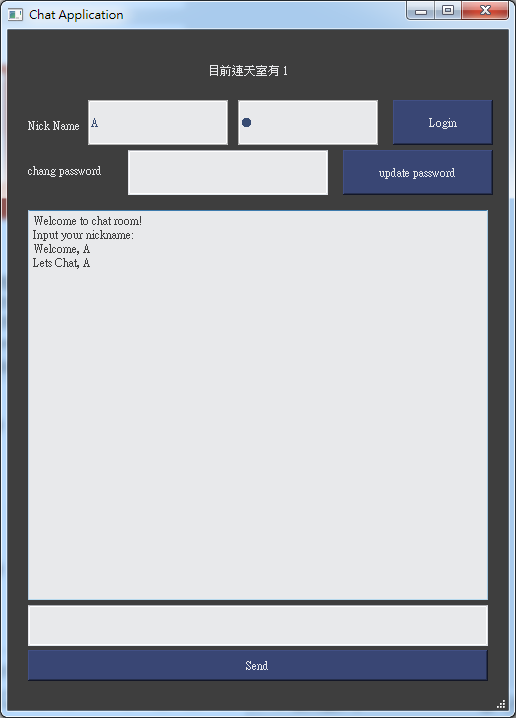
\includegraphics[scale=0.35]{clientui}
\end{frame}

\begin{frame}[t]
\frametitle{\huge Client端功能} % Table of contents slide
\begin{itemize}
\Large \item 登入
\item 改密碼
\item 發送訊息
\item 顯示其他client端的訊息
\end{itemize}
\end{frame}

\begin{frame}
\frametitle{\huge Sever端介面} % Table of contents slide
\hspace{3.5cm} 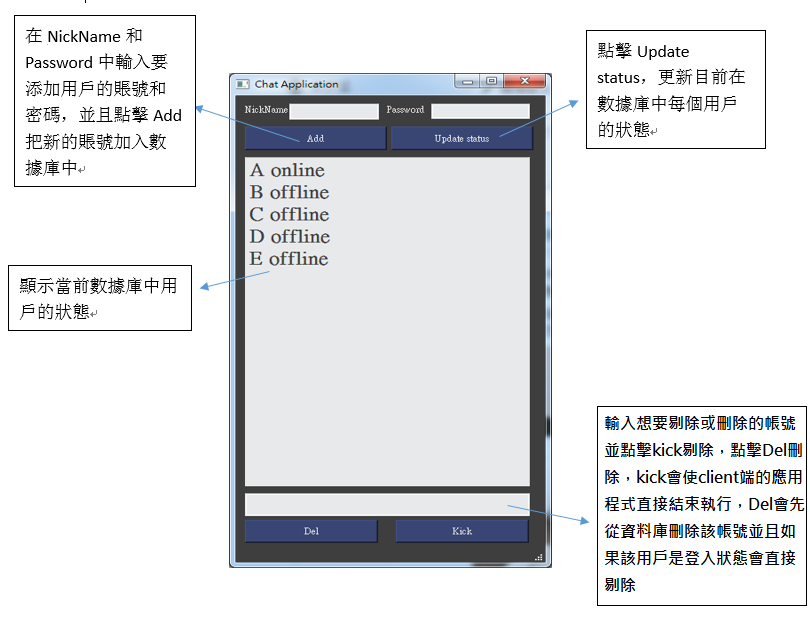
\includegraphics[scale=0.4]{serverui}
\end{frame}

\begin{frame}[t]
\frametitle{\huge Sever端功能} % Table of contents slide
\begin{itemize}
\Large \item 增加帳密
\item 刪除帳戶
\item 顯示用戶是否在線上
\item 處理bot天氣、匯率
\end{itemize}
\end{frame}

\begin{frame}[t]
\frametitle{\LARGE MongoDB} % Table of contents slide
\hspace{0.5cm} 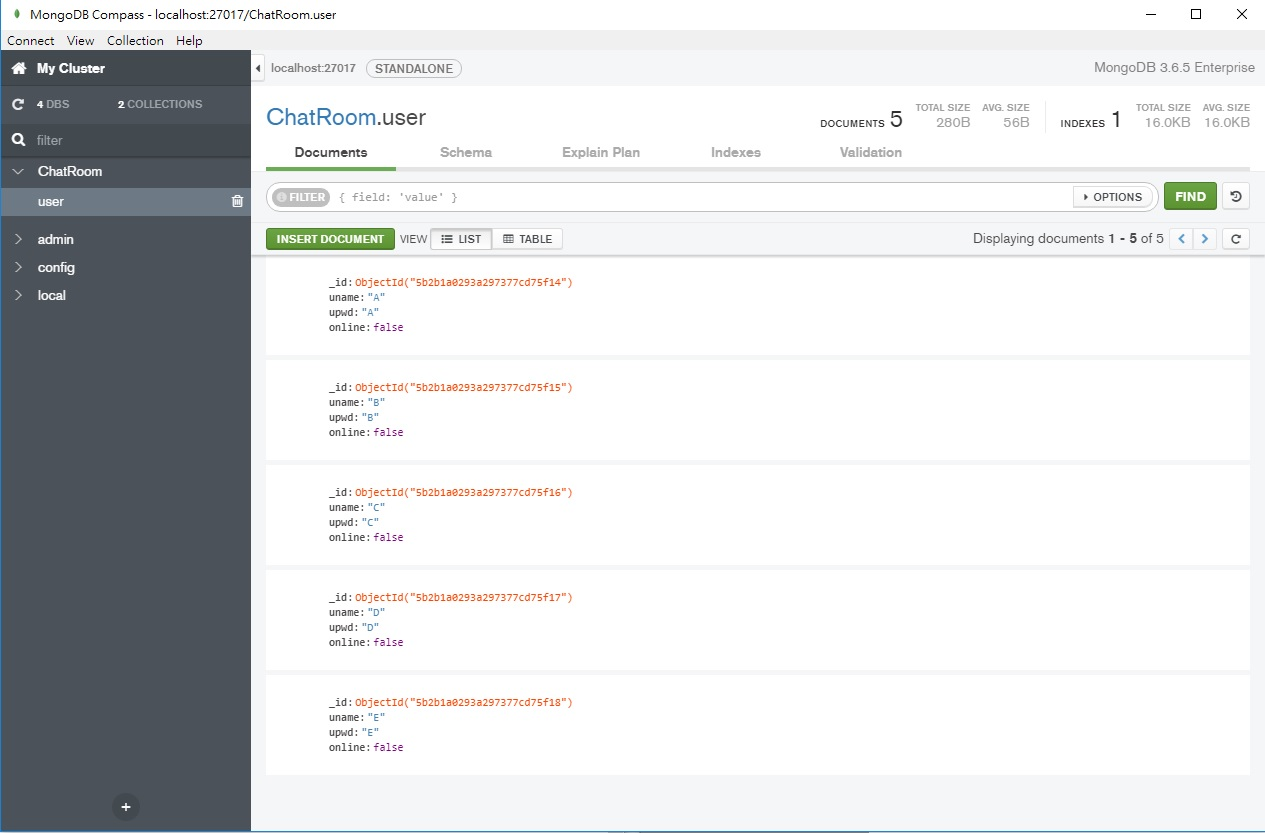
\includegraphics[scale=0.3]{mongodb}
\end{frame}
%----------------------------------------------------------------------------------------
\begin{frame}[t]
\frametitle{\huge 系統結構圖} % Table of contents slide
\hspace{3em}  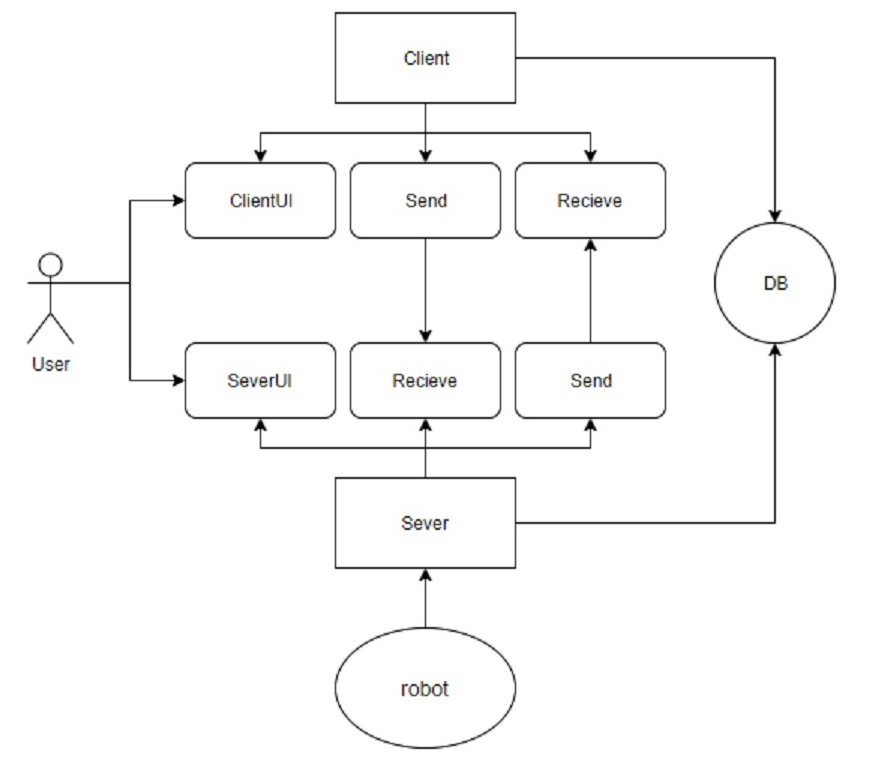
\includegraphics[scale=0.35]{sad}
\end{frame}

\begin{frame}[t]
\frametitle{\LARGE 實作方法} % Table of contents slide
\vspace{2em}
\hspace{2em} \Large 利用Socket通訊,開啟Sever後,Client傳送訊息,再利用Server廣播給其他Client,Client登錄時,會傳送一個特殊碼給Server,Server就會計算在線人數,回傳給所有的Client。
\end{frame}

\begin{frame}[t]
\vspace{1.5em}
\frametitle{\LARGE 實作方法} % Table of contents slide
\hspace{2em} \Large 偵測發送的訊息,判斷是否是給bot的指令,若是的話,則會利用api找到答案,並回傳給所有的Client。
\vspace{6em}
\hspace{4em} 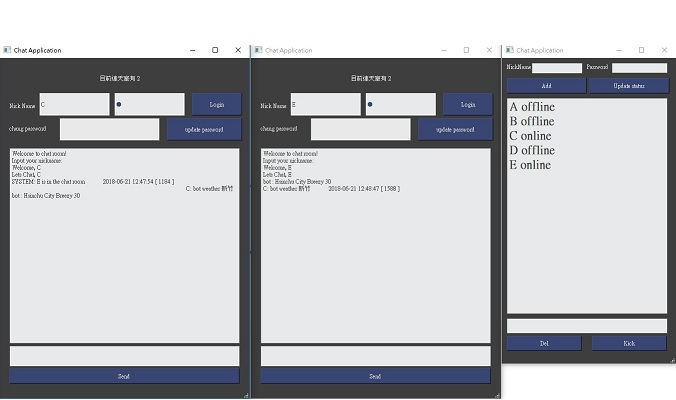
\includegraphics[scale=0.4]{figure1}
\end{frame}


%----------------------------------------------------------------------------------------
\begin{frame}
\frametitle{\LARGE DEMO} % Table of contents slide
\centerline{\LARGE 實際示範}
\end{frame}
%----------------------------------------------------------------------------------------
\begin{frame}[t]
\frametitle{\huge Revision History} % Table of contents slide
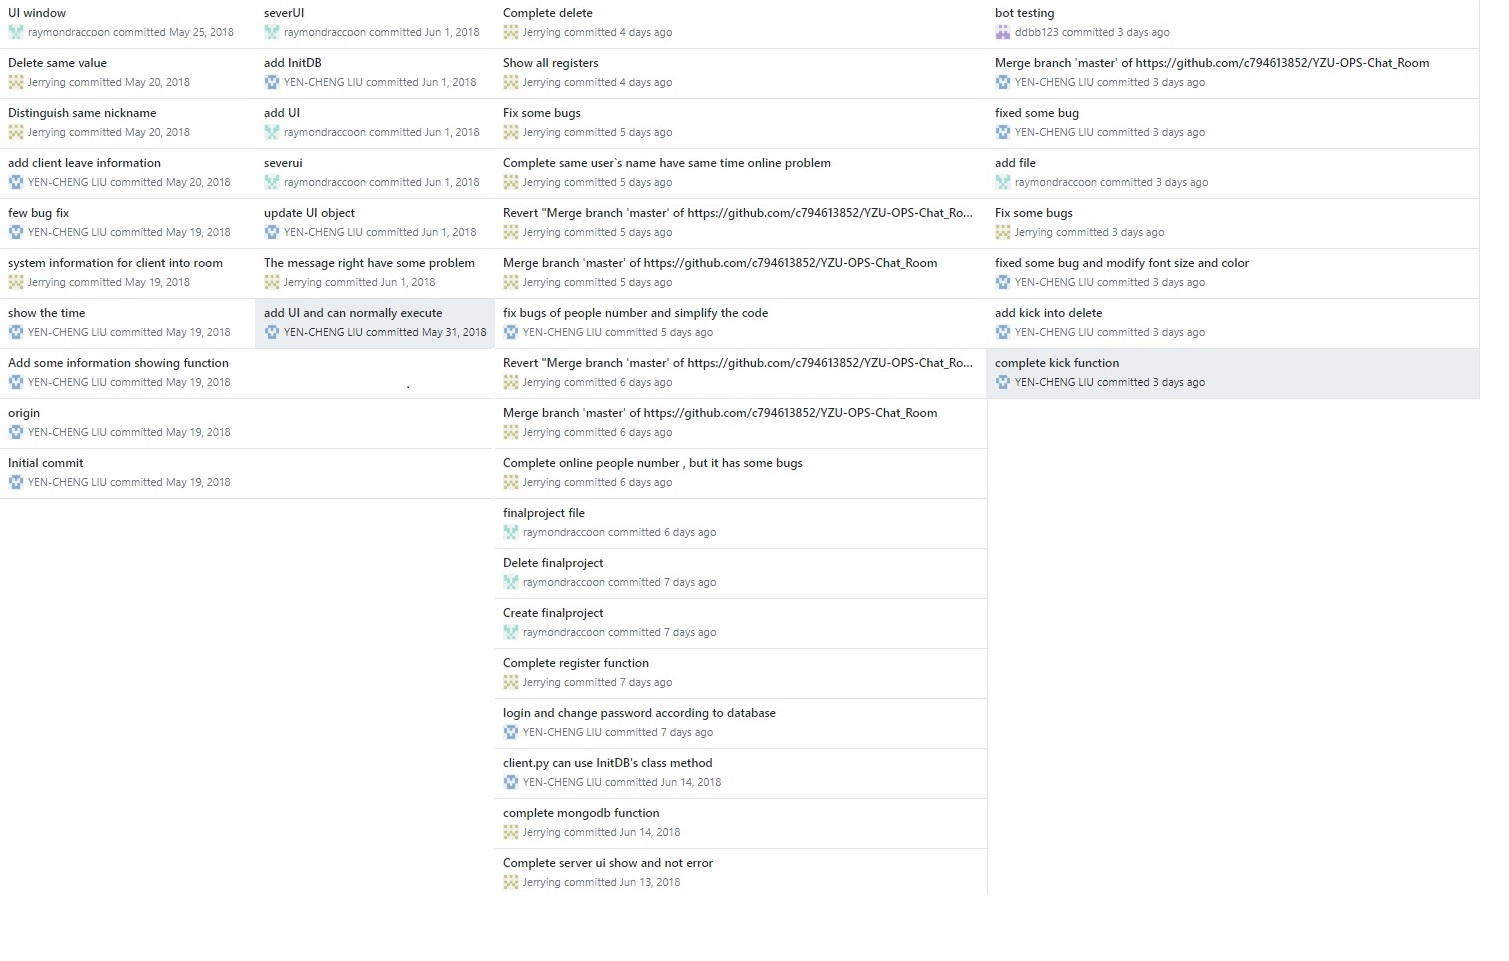
\includegraphics[scale=0.3]{history}
\end{frame}
%----------------------------------------------------------------------------------------

\end{document}

